\documentclass[../../project.tex]{subfiles}
\graphicspath{{\subfix{images/}}}

\begin{document}
	The given dataset was bootstrapped 400 times and both DA models were tested before and after input transformations.
	\begin{table}[h!]
		\centering
		\begin{tabular}{cccc}
			Input & DA Model & Mean Accuracy & Mean AUC \\
			\midrule
			Before transformations
			& LDA & 0.856 & 0.870 \\
		    & QDA & 0.818 & 0.849 \\
			\midrule
			After transformations
			& LDA & 0.893 & 0.913 \\
			& QDA & 0.933 & 0.966 \\
		\end{tabular}
		\caption{Mean Accuracy and Mean AUC for discriminant analysis models. 70\% training data.}
		\label{tab:discanal_table_70}
	\end{table}
	\begin{table}[h!]
		\centering
		\begin{tabular}{cccc}
			Input & DA Model & Mean Accuracy & Mean AUC \\
			\midrule
			Before transformations
			& LDA & 0.866 & 0.877 \\
		    & QDA & 0.840 & 0.869 \\
			\midrule
			After transformations
			& LDA & 0.903 & 0.915 \\
			& QDA & 0.942 & 0.977 \\
		\end{tabular}
		\caption{Mean Accuracy and Mean AUC for discriminant analysis models. 90\% training data.}
		\label{tab:discanal_table_90}
	\end{table}
	From the results it is clear that QDA seems to have better performance after transformations. It is unclear which method performs better before the transformation because for QDA the variance is high. The high variance can for QDA can be explained by the fact that the original inputs are close to being colinear making $\Sigma$ close to being singular which in turn results in an inaccurate matrix inversion. For example, the standard deviation of accuracy and AUC of the QDA classifier, before transformations, on 400 bootstrapped datasets with 90\% training data were 0.076 and 0.081 respectively compared to 0.021 and 0.019 after transformations ceteris paribus.
	
	Cross validation was carried out to estimate the accuracy using 150 folds resulting in an estimated accuracy of 0.948. As can be seen in table \ref{tbl:boxplotQDA} the 
	
	One problem with the QDA model was however the outliers170seen in the boxplot of 3.3. Similar outliers were found in the case ofk-NN and logistic regression171these could probably be explained by the occurrence of a "bad split" where for example many movies172deviating from the average movie end up in the test portion resulting in a bad performance.
	
	\begin{table}[]
		\centering
    	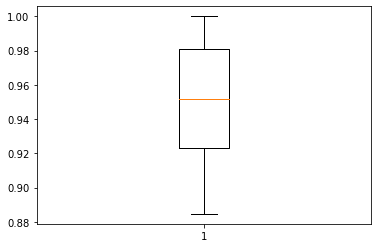
\includegraphics[scale=0.7]{project/tex/QDAboxplot.png}
		\caption{Accuracy estimation using cross validation with 150 folds.}
		\label{tbl:boxplotQDA}
    \end{table}
    
    
	--Based on the results it seems that LDA is not complex enough of a model for this task. SKRIV OM VARFÖR QDA ÄR BÄTTRE ÄN LDA FÖR DET HÄR

	-- några fall av väldigt dåliga resultat (70-75\%) går detta att undvika? har johannes modell lika? är det pga otur i uppdelningen av datan vid cross validation??
	-- 0.9428 accuracy cross validation 100 folds 70\% training data
	-- ENDAST EFTER TRANSFORMATION
	-- 0.9420 accuracy cross validation 100 folds 90\% training data
	
	-Model accuracy change after transformation QuadraticDiscriminantAnalysis() is 
0.007000000000000029 efter att ha tagit bort gross och year från transformerade datan
-Model accuracy change after transformation QuadraticDiscriminantAnalysis() is 
0.09036363636363674 slutliga inputs jämfört med original inputsen
\end{document}